\section{Design}
Snake-spillet er lavet efter et \textit{Model-View-Controller}-design (MVC). Styringen, spil-logikken og den visuelle repræsentation holdes adskilt i tre dele. Med dette bygges et meget modulært program. Spil-logikken er \textit{Model}, styringen er \textit{Control} og den visuelle repræsentation er \textit{View}. Disse tre dele skal kode-mæssigt holdes adskilt. Spil-logikken må ikke kende til styringen eller den visuelle repræsentation, mens den visuelle repræsentation godt må kende til spil-logikken, men ikke til styringen. Styringen må kende til både spil-logikken og den visuelle repræsentation (se \figref{mvc}).
\newline

\begin{figure}[h]
	\centering
   	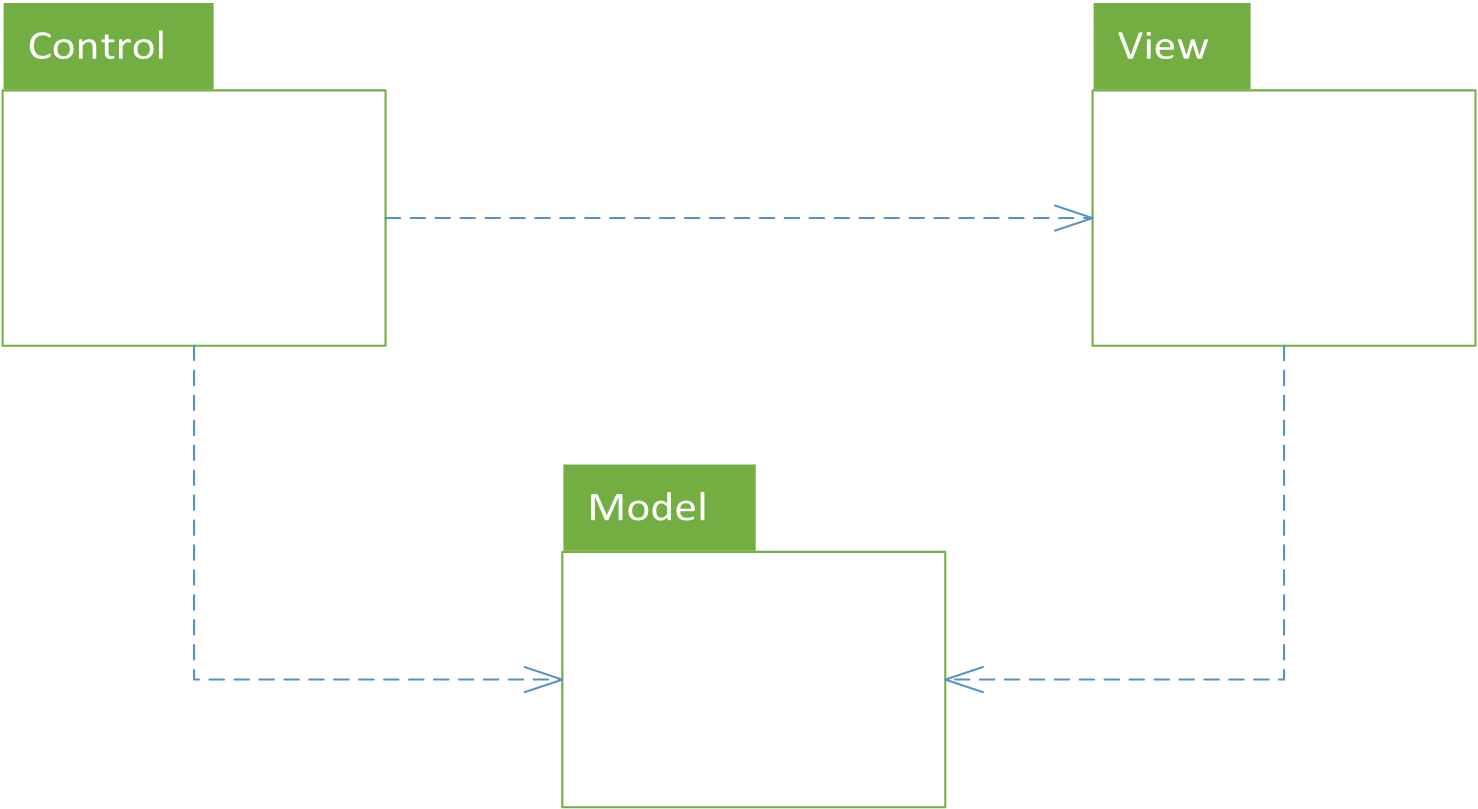
\includegraphics[width=0.7\textwidth]{grundlaeggende/mvc.png}

	\caption{\figlab{mvc}\textit{Oversigt over Model-View-Controller-designet.}}
\end{figure}

På denne måde interagerer brugeren kun med den del af programmet, der er dedikeret til styring. Styringen manipulerer programmets tilstand i \textit{model}-koden, som visualiseres i \textit{view}-koden. Dette betyder derfor også, at alle funktioner, der påvirker programmets tilstand, skal holdes i \textit{model}-koden. \textit{Control} modtager kun input fra brugeren, og sender dette videre til \textit{View} og \textit{Model}. Det er muligt gennem en Observer at "observere" ændringerne i spillet, som derefter opdateres i \textit{View} (se Appendix A for UML klassediagrammer).
\newline

Simple Snake er designet, så spillets logik ligger i klassen \textit{Game} i model-pakken. \textit{Game} får da spillets objekter fra andre klasser i \textit{model}-pakken, f.eks. \textit{Food} og \textit{Snake}. Enumerations-klassen, \textit{Direction}, forsimpler kommunikation med \textit{Game}-klassen, idet det er nemmere at tilkoble en masse kommandoer og statements til hver retning, hvis der eksplicit er en \textit{Direction}-klasse, som begrænser retningsmulighederne. Vi har valgt at gøre \textit{Game} til en Observable klasse, da view-klasserne derved kan observere model-delen og opdatere brugergrænsefladen, så snart spillets tilstand ændrer sig. \textit{Snake}-klassen afhænger af \textit{Game}-klassen, da 'move'-metoden i \textit{Snake} er nødt til at signalere til \textit{Game}, at slangen har bevæget sig. Dette gør den ved at kalde på den 'snakeHasMoved'-metode.

I view-pakken ligger \textit{View}, der er vinduet, som spilleren ser spillet igennem. Det er her \textit{BoardPanel}-klassen, der viser den nuværende spil-tilstand. Denne er en Observer, som notificeres hver gang banens tilstand ændres i modellen. Når dette sker, eller når spillet startes, tegnes banen, slangen og maden fra \textit{Game}-klassen, vha. klasserne \textit{View} og \textit{BoardPanel}. Scoren holdes i \textit{Game}-klassen og vises i view-klassen \textit{ScorePanel}. Dette panel er placeret over \textit{BoardPanel} i \textit{View}-vinduet. Den observerer \textit{Game}, og opdaterer sig selv, når scoren ændrer sig.

\textit{Control}-klassen kalder relevante \textit{Game}- og \textit{Snake}-metoder når spilleren trykker på tastaturet. Klassen nedarver fra KeyListener og bestemmer hvornår og hvorhen slangen skal bevæge sig.

For at starte spillet bruges klassen \textit{Driver}, som opretter et nyt \textit{Game}-, \textit{View} og \textit{Control}-objekt.